\documentclass{standalone}
\usepackage{tikz}
\usetikzlibrary{patterns}
\usetikzlibrary{positioning}
\usetikzlibrary{patterns, positioning}
\usetikzlibrary{shapes.misc}
\usepackage[outline]{contour}
\contourlength{1.5pt} 
\usetikzlibrary{calc}
        \usepackage{relsize}
        \tikzset{fontscale/.style = {font=\relsize{#1}}}

\begin{document}
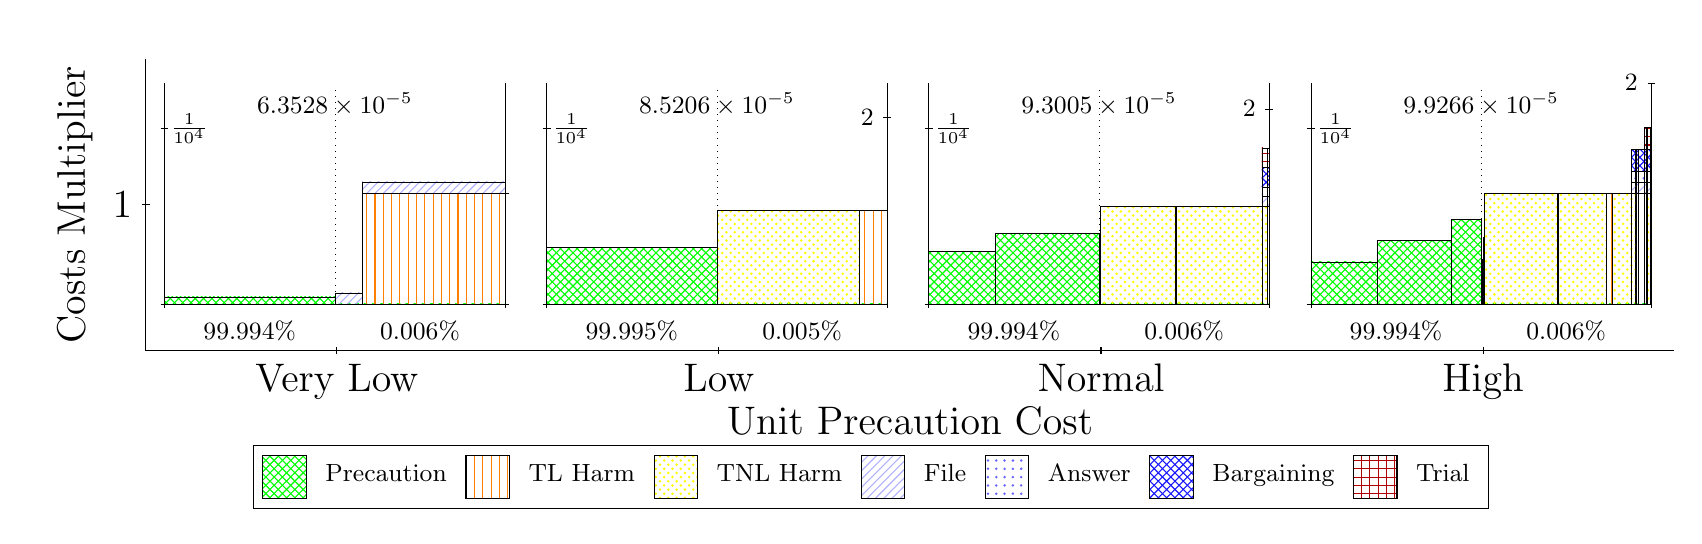
\begin{tikzpicture}
\clip(-0.5,-1.1) rectangle +(20.91,6.2);
\draw[black] (1,1) -- (1,4.7);
\node[rotate=90, fontscale=2, anchor=center] at (0.1, 2.85) {Costs Multiplier};
\draw[black] (0.95,2.85) -- (1.05,2.85);
\node[fontscale=2, anchor=east] at (0.95, 2.85) {1};

\draw[black] (1,1) -- (20.41,1);
\node[fontscale=2, anchor=center] at (10.705, 0.1) {Unit Precaution Cost};
\draw[black] (3.4263,0.95) -- (3.4263,1.05);
\node[fontscale=2, anchor=north] at (3.4263, 0.95) {Very Low};
\draw[black] (8.2788,0.95) -- (8.2788,1.05);
\node[fontscale=2, anchor=north] at (8.2788, 0.95) {Low};
\draw[black] (13.131,0.95) -- (13.131,1.05);
\node[fontscale=2, anchor=north] at (13.131, 0.95) {Normal};
\draw[black] (17.984,0.95) -- (17.984,1.05);
\node[fontscale=2, anchor=north] at (17.984, 0.95) {High};


\draw[pattern=crosshatch, pattern color=green,draw=black,very thin] (1.2381,1.592) rectangle (3.4013,1.6811);
\draw[pattern=crosshatch, pattern color=green,draw=black,very thin] (3.4013,1.592) rectangle (3.7435,1.592);
\draw[pattern=north east lines, pattern color=blue!30,draw=black,very thin] (3.4013,1.592) rectangle (3.7435,1.7328);
\draw[pattern=crosshatch, pattern color=green,draw=black,very thin] (3.7435,1.592) rectangle (5.5644,1.592);
\draw[pattern=vertical lines, pattern color=orange,draw=black,very thin] (3.7435,1.592) rectangle (5.5644,3);
\draw[pattern=north east lines, pattern color=blue!30,draw=black,very thin] (3.7435,3) rectangle (5.5644,3.1408);
\node[font=\small,text=black,anchor=north] at (3.4013, 4.4) {$6.3528\times 10^{-5}$};
\draw[black,very thin] (1.2381,1.592) -- (1.2381,4.4);
\draw[black,very thin] (1.1881,1.592) -- (1.2881,1.592);
\node[font=\small,text=black, anchor=west] at (1.1881, 1.592) {};
\draw[black,very thin] (1.1881,3.8194) -- (1.2881,3.8194);
\node[font=\small,text=black, anchor=west] at (1.1881, 3.8194) {$\frac{1}{10^{4}}$};

\draw[black,dotted,very thin] (3.4013,1.6762) -- (3.4013,4.3158);
\draw[black,very thin] (5.5644,1.592) -- (5.5644,4.4);
\draw[black,very thin] (5.5144,1.592) -- (5.6144,1.592);
\node[font=\small,text=black, anchor=east] at (5.5144, 1.592) {\contour{white}{}};
\draw[black,very thin] (5.5144,3) -- (5.6144,3);
\node[font=\small,text=black, anchor=east] at (5.5144, 3) {\contour{white}{}};

\draw[black,very thin] (1.2381,1.592) -- (5.5644,1.592);
\draw[black,very thin] (1.2381,1.542) -- (1.2381,1.642);
\node[font=\small,text=black, anchor=north] at (1.2381, 1.542) {};
\draw[black,very thin] (5.5644,1.542) -- (5.5644,1.642);
\node[font=\small,text=black, anchor=north] at (5.5644, 1.542) {};

\node[font=\small,text=black,anchor=south] at (2.3197, 0.992) {99.994\%};
\node[font=\small,text=black,anchor=south] at (4.4828, 0.992) {0.006\%};

\draw[pattern=crosshatch, pattern color=green,draw=black,very thin] (6.0906,1.592) rectangle (8.2538,2.3048);
\draw[pattern=crosshatch, pattern color=green,draw=black,very thin] (8.2538,1.592) rectangle (10.066,1.592);
\draw[pattern=crosshatch dots, pattern color=yellow,draw=black,very thin] (8.2538,1.592) rectangle (10.066,2.7772);
\draw[pattern=crosshatch, pattern color=green,draw=black,very thin] (10.066,1.592) rectangle (10.417,1.592);
\draw[pattern=vertical lines, pattern color=orange,draw=black,very thin] (10.066,1.592) rectangle (10.417,2.7772);
\node[font=\small,text=black,anchor=north] at (8.2538, 4.4) {$8.5206\times 10^{-5}$};
\draw[black,very thin] (6.0906,1.592) -- (6.0906,4.4);
\draw[black,very thin] (6.0406,1.592) -- (6.1406,1.592);
\node[font=\small,text=black, anchor=west] at (6.0406, 1.592) {};
\draw[black,very thin] (6.0406,3.8194) -- (6.1406,3.8194);
\node[font=\small,text=black, anchor=west] at (6.0406, 3.8194) {$\frac{1}{10^{4}}$};

\draw[black,dotted,very thin] (8.2538,1.6762) -- (8.2538,4.3158);
\draw[black,very thin] (10.417,1.592) -- (10.417,4.4);
\draw[black,very thin] (10.367,3.9624) -- (10.467,3.9624);
\node[font=\small,text=black, anchor=east] at (10.367, 3.9624) {\contour{white}{2}};

\draw[black,very thin] (6.0906,1.592) -- (10.417,1.592);
\draw[black,very thin] (6.0906,1.542) -- (6.0906,1.642);
\node[font=\small,text=black, anchor=north] at (6.0906, 1.542) {};
\draw[black,very thin] (10.417,1.542) -- (10.417,1.642);
\node[font=\small,text=black, anchor=north] at (10.417, 1.542) {};

\node[font=\small,text=black,anchor=south] at (7.1722, 0.992) {99.995\%};
\node[font=\small,text=black,anchor=south] at (9.3353, 0.992) {0.005\%};

\draw[pattern=crosshatch, pattern color=green,draw=black,very thin] (10.943,1.592) rectangle (11.791,2.2602);
\draw[pattern=crosshatch, pattern color=green,draw=black,very thin] (11.791,1.592) rectangle (13.106,2.483);
\draw[pattern=crosshatch, pattern color=green,draw=black,very thin] (13.106,1.592) rectangle (13.122,1.592);
\draw[pattern=north east lines, pattern color=blue!30,draw=black,very thin] (13.106,1.592) rectangle (13.122,1.7159);
\draw[pattern=dots,  pattern color=blue!60,draw=black,very thin] (13.106,1.7159) rectangle (13.122,1.8398);
\draw[pattern=crosshatch,      pattern color=blue!90,draw=black,very thin] (13.106,1.8398) rectangle (13.122,2.0875);
\draw[pattern=grid,            pattern color=red!70!black,draw=black,very thin] (13.106,2.0875) rectangle (13.122,2.3352);
\draw[pattern=crosshatch, pattern color=green,draw=black,very thin] (13.122,1.592) rectangle (14.072,1.592);
\draw[pattern=crosshatch dots, pattern color=yellow,draw=black,very thin] (13.122,1.592) rectangle (14.072,2.8307);
\draw[pattern=crosshatch, pattern color=green,draw=black,very thin] (14.072,1.592) rectangle (14.082,1.592);
\draw[pattern=vertical lines, pattern color=orange,draw=black,very thin] (14.072,1.592) rectangle (14.082,2.8307);
\draw[pattern=crosshatch, pattern color=green,draw=black,very thin] (14.082,1.592) rectangle (15.173,1.592);
\draw[pattern=crosshatch dots, pattern color=yellow,draw=black,very thin] (14.082,1.592) rectangle (15.173,2.8307);
\draw[pattern=crosshatch, pattern color=green,draw=black,very thin] (15.173,1.592) rectangle (15.244,1.592);
\draw[pattern=crosshatch dots, pattern color=yellow,draw=black,very thin] (15.173,1.592) rectangle (15.244,2.8307);
\draw[pattern=north east lines, pattern color=blue!30,draw=black,very thin] (15.173,2.8307) rectangle (15.244,2.9545);
\draw[pattern=dots,  pattern color=blue!60,draw=black,very thin] (15.173,2.9545) rectangle (15.244,3.0784);
\draw[pattern=crosshatch,      pattern color=blue!90,draw=black,very thin] (15.173,3.0784) rectangle (15.244,3.3261);
\draw[pattern=grid,            pattern color=red!70!black,draw=black,very thin] (15.173,3.3261) rectangle (15.244,3.5738);
\draw[pattern=crosshatch, pattern color=green,draw=black,very thin] (15.244,1.592) rectangle (15.269,1.592);
\draw[pattern=vertical lines, pattern color=orange,draw=black,very thin] (15.244,1.592) rectangle (15.269,2.8307);
\draw[pattern=north east lines, pattern color=blue!30,draw=black,very thin] (15.244,2.8307) rectangle (15.269,2.9545);
\draw[pattern=dots,  pattern color=blue!60,draw=black,very thin] (15.244,2.9545) rectangle (15.269,3.0784);
\draw[pattern=crosshatch,      pattern color=blue!90,draw=black,very thin] (15.244,3.0784) rectangle (15.269,3.3261);
\draw[pattern=grid,            pattern color=red!70!black,draw=black,very thin] (15.244,3.3261) rectangle (15.269,3.5738);
\node[font=\small,text=black,anchor=north] at (13.106, 4.4) {$9.3005\times 10^{-5}$};
\draw[black,very thin] (10.943,1.592) -- (10.943,4.4);
\draw[black,very thin] (10.893,1.592) -- (10.993,1.592);
\node[font=\small,text=black, anchor=west] at (10.893, 1.592) {};
\draw[black,very thin] (10.893,3.8194) -- (10.993,3.8194);
\node[font=\small,text=black, anchor=west] at (10.893, 3.8194) {$\frac{1}{10^{4}}$};

\draw[black,dotted,very thin] (13.106,1.6762) -- (13.106,4.3158);
\draw[black,very thin] (15.269,1.592) -- (15.269,4.4);
\draw[black,very thin] (15.219,4.0692) -- (15.319,4.0692);
\node[font=\small,text=black, anchor=east] at (15.219, 4.0692) {\contour{white}{2}};

\draw[black,very thin] (10.943,1.592) -- (15.269,1.592);
\draw[black,very thin] (10.943,1.542) -- (10.943,1.642);
\node[font=\small,text=black, anchor=north] at (10.943, 1.542) {};
\draw[black,very thin] (15.269,1.542) -- (15.269,1.642);
\node[font=\small,text=black, anchor=north] at (15.269, 1.542) {};

\node[font=\small,text=black,anchor=south] at (12.025, 0.992) {99.994\%};
\node[font=\small,text=black,anchor=south] at (14.188, 0.992) {0.006\%};

\draw[pattern=crosshatch, pattern color=green,draw=black,very thin] (15.796,1.592) rectangle (16.643,2.1266);
\draw[pattern=crosshatch, pattern color=green,draw=black,very thin] (16.643,1.592) rectangle (17.578,2.3939);
\draw[pattern=crosshatch, pattern color=green,draw=black,very thin] (17.578,1.592) rectangle (17.959,2.6612);
\draw[pattern=crosshatch, pattern color=green,draw=black,very thin] (17.959,1.592) rectangle (17.967,1.592);
\draw[pattern=north east lines, pattern color=blue!30,draw=black,very thin] (17.959,1.592) rectangle (17.967,1.7324);
\draw[pattern=dots,  pattern color=blue!60,draw=black,very thin] (17.959,1.7324) rectangle (17.967,1.8728);
\draw[pattern=crosshatch,      pattern color=blue!90,draw=black,very thin] (17.959,1.8728) rectangle (17.967,2.1536);
\draw[pattern=crosshatch, pattern color=green,draw=black,very thin] (17.967,1.592) rectangle (17.989,1.5921);
\draw[pattern=north east lines, pattern color=blue!30,draw=black,very thin] (17.967,1.5921) rectangle (17.989,1.7324);
\draw[pattern=dots,  pattern color=blue!60,draw=black,very thin] (17.967,1.7324) rectangle (17.989,1.8728);
\draw[pattern=crosshatch,      pattern color=blue!90,draw=black,very thin] (17.967,1.8728) rectangle (17.989,2.1536);
\draw[pattern=crosshatch, pattern color=green,draw=black,very thin] (17.989,1.592) rectangle (17.995,1.592);
\draw[pattern=north east lines, pattern color=blue!30,draw=black,very thin] (17.989,1.592) rectangle (17.995,1.7324);
\draw[pattern=dots,  pattern color=blue!60,draw=black,very thin] (17.989,1.7324) rectangle (17.995,1.8728);
\draw[pattern=crosshatch,      pattern color=blue!90,draw=black,very thin] (17.989,1.8728) rectangle (17.995,2.1536);
\draw[pattern=grid,            pattern color=red!70!black,draw=black,very thin] (17.989,2.1536) rectangle (17.995,2.4344);
\draw[pattern=crosshatch, pattern color=green,draw=black,very thin] (17.995,1.592) rectangle (18.004,1.5921);
\draw[pattern=north east lines, pattern color=blue!30,draw=black,very thin] (17.995,1.5921) rectangle (18.004,1.7324);
\draw[pattern=dots,  pattern color=blue!60,draw=black,very thin] (17.995,1.7324) rectangle (18.004,1.8728);
\draw[pattern=crosshatch,      pattern color=blue!90,draw=black,very thin] (17.995,1.8728) rectangle (18.004,2.1536);
\draw[pattern=grid,            pattern color=red!70!black,draw=black,very thin] (17.995,2.1536) rectangle (18.004,2.4344);
\draw[pattern=crosshatch, pattern color=green,draw=black,very thin] (18.004,1.592) rectangle (18.931,1.592);
\draw[pattern=crosshatch dots, pattern color=yellow,draw=black,very thin] (18.004,1.592) rectangle (18.931,2.996);
\draw[pattern=crosshatch, pattern color=green,draw=black,very thin] (18.931,1.592) rectangle (18.94,1.592);
\draw[pattern=vertical lines, pattern color=orange,draw=black,very thin] (18.931,1.592) rectangle (18.94,2.996);
\draw[pattern=crosshatch, pattern color=green,draw=black,very thin] (18.94,1.592) rectangle (19.55,1.5921);
\draw[pattern=crosshatch dots, pattern color=yellow,draw=black,very thin] (18.94,1.5921) rectangle (19.55,2.996);
\draw[pattern=crosshatch, pattern color=green,draw=black,very thin] (19.55,1.592) rectangle (19.627,1.5921);
\draw[pattern=vertical lines, pattern color=orange,draw=black,very thin] (19.55,1.5921) rectangle (19.627,2.996);
\draw[pattern=crosshatch, pattern color=green,draw=black,very thin] (19.627,1.592) rectangle (19.865,1.5921);
\draw[pattern=crosshatch dots, pattern color=yellow,draw=black,very thin] (19.627,1.5921) rectangle (19.865,2.996);
\draw[pattern=crosshatch, pattern color=green,draw=black,very thin] (19.865,1.592) rectangle (19.91,1.592);
\draw[pattern=crosshatch dots, pattern color=yellow,draw=black,very thin] (19.865,1.592) rectangle (19.91,2.996);
\draw[pattern=north east lines, pattern color=blue!30,draw=black,very thin] (19.865,2.996) rectangle (19.91,3.1364);
\draw[pattern=dots,  pattern color=blue!60,draw=black,very thin] (19.865,3.1364) rectangle (19.91,3.2768);
\draw[pattern=crosshatch,      pattern color=blue!90,draw=black,very thin] (19.865,3.2768) rectangle (19.91,3.5576);
\draw[pattern=crosshatch, pattern color=green,draw=black,very thin] (19.91,1.592) rectangle (19.923,1.592);
\draw[pattern=vertical lines, pattern color=orange,draw=black,very thin] (19.91,1.592) rectangle (19.923,2.996);
\draw[pattern=north east lines, pattern color=blue!30,draw=black,very thin] (19.91,2.996) rectangle (19.923,3.1364);
\draw[pattern=dots,  pattern color=blue!60,draw=black,very thin] (19.91,3.1364) rectangle (19.923,3.2768);
\draw[pattern=crosshatch,      pattern color=blue!90,draw=black,very thin] (19.91,3.2768) rectangle (19.923,3.5576);
\draw[pattern=crosshatch, pattern color=green,draw=black,very thin] (19.923,1.592) rectangle (19.959,1.5921);
\draw[pattern=crosshatch dots, pattern color=yellow,draw=black,very thin] (19.923,1.5921) rectangle (19.959,2.996);
\draw[pattern=north east lines, pattern color=blue!30,draw=black,very thin] (19.923,2.996) rectangle (19.959,3.1364);
\draw[pattern=dots,  pattern color=blue!60,draw=black,very thin] (19.923,3.1364) rectangle (19.959,3.2768);
\draw[pattern=crosshatch,      pattern color=blue!90,draw=black,very thin] (19.923,3.2768) rectangle (19.959,3.5576);
\draw[pattern=crosshatch, pattern color=green,draw=black,very thin] (19.959,1.592) rectangle (20.03,1.5921);
\draw[pattern=vertical lines, pattern color=orange,draw=black,very thin] (19.959,1.5921) rectangle (20.03,2.996);
\draw[pattern=north east lines, pattern color=blue!30,draw=black,very thin] (19.959,2.996) rectangle (20.03,3.1364);
\draw[pattern=dots,  pattern color=blue!60,draw=black,very thin] (19.959,3.1364) rectangle (20.03,3.2768);
\draw[pattern=crosshatch,      pattern color=blue!90,draw=black,very thin] (19.959,3.2768) rectangle (20.03,3.5576);
\draw[pattern=crosshatch, pattern color=green,draw=black,very thin] (20.03,1.592) rectangle (20.06,1.592);
\draw[pattern=crosshatch dots, pattern color=yellow,draw=black,very thin] (20.03,1.592) rectangle (20.06,2.996);
\draw[pattern=north east lines, pattern color=blue!30,draw=black,very thin] (20.03,2.996) rectangle (20.06,3.1364);
\draw[pattern=dots,  pattern color=blue!60,draw=black,very thin] (20.03,3.1364) rectangle (20.06,3.2768);
\draw[pattern=crosshatch,      pattern color=blue!90,draw=black,very thin] (20.03,3.2768) rectangle (20.06,3.5576);
\draw[pattern=grid,            pattern color=red!70!black,draw=black,very thin] (20.03,3.5576) rectangle (20.06,3.8384);
\draw[pattern=crosshatch, pattern color=green,draw=black,very thin] (20.06,1.592) rectangle (20.071,1.592);
\draw[pattern=vertical lines, pattern color=orange,draw=black,very thin] (20.06,1.592) rectangle (20.071,2.996);
\draw[pattern=north east lines, pattern color=blue!30,draw=black,very thin] (20.06,2.996) rectangle (20.071,3.1364);
\draw[pattern=dots,  pattern color=blue!60,draw=black,very thin] (20.06,3.1364) rectangle (20.071,3.2768);
\draw[pattern=crosshatch,      pattern color=blue!90,draw=black,very thin] (20.06,3.2768) rectangle (20.071,3.5576);
\draw[pattern=grid,            pattern color=red!70!black,draw=black,very thin] (20.06,3.5576) rectangle (20.071,3.8384);
\draw[pattern=crosshatch, pattern color=green,draw=black,very thin] (20.071,1.592) rectangle (20.103,1.5921);
\draw[pattern=crosshatch dots, pattern color=yellow,draw=black,very thin] (20.071,1.5921) rectangle (20.103,2.996);
\draw[pattern=north east lines, pattern color=blue!30,draw=black,very thin] (20.071,2.996) rectangle (20.103,3.1364);
\draw[pattern=dots,  pattern color=blue!60,draw=black,very thin] (20.071,3.1364) rectangle (20.103,3.2768);
\draw[pattern=crosshatch,      pattern color=blue!90,draw=black,very thin] (20.071,3.2768) rectangle (20.103,3.5576);
\draw[pattern=grid,            pattern color=red!70!black,draw=black,very thin] (20.071,3.5576) rectangle (20.103,3.8384);
\draw[pattern=crosshatch, pattern color=green,draw=black,very thin] (20.103,1.592) rectangle (20.122,1.5921);
\draw[pattern=vertical lines, pattern color=orange,draw=black,very thin] (20.103,1.5921) rectangle (20.122,2.996);
\draw[pattern=north east lines, pattern color=blue!30,draw=black,very thin] (20.103,2.996) rectangle (20.122,3.1364);
\draw[pattern=dots,  pattern color=blue!60,draw=black,very thin] (20.103,3.1364) rectangle (20.122,3.2768);
\draw[pattern=crosshatch,      pattern color=blue!90,draw=black,very thin] (20.103,3.2768) rectangle (20.122,3.5576);
\draw[pattern=grid,            pattern color=red!70!black,draw=black,very thin] (20.103,3.5576) rectangle (20.122,3.8384);
\node[font=\small,text=black,anchor=north] at (17.959, 4.4) {$9.9266\times 10^{-5}$};
\draw[black,very thin] (15.796,1.592) -- (15.796,4.4);
\draw[black,very thin] (15.746,1.592) -- (15.846,1.592);
\node[font=\small,text=black, anchor=west] at (15.746, 1.592) {};
\draw[black,very thin] (15.746,3.8194) -- (15.846,3.8194);
\node[font=\small,text=black, anchor=west] at (15.746, 3.8194) {$\frac{1}{10^{4}}$};

\draw[black,dotted,very thin] (17.959,1.6762) -- (17.959,4.3158);
\draw[black,very thin] (20.122,1.592) -- (20.122,4.4);
\draw[black,very thin] (20.072,4.3999) -- (20.172,4.3999);
\node[font=\small,text=black, anchor=east] at (20.072, 4.3999) {\contour{white}{2}};

\draw[black,very thin] (15.796,1.592) -- (20.122,1.592);
\draw[black,very thin] (15.796,1.542) -- (15.796,1.642);
\node[font=\small,text=black, anchor=north] at (15.796, 1.542) {};
\draw[black,very thin] (20.122,1.542) -- (20.122,1.642);
\node[font=\small,text=black, anchor=north] at (20.122, 1.542) {};

\node[font=\small,text=black,anchor=south] at (16.877, 0.992) {99.994\%};
\node[font=\small,text=black,anchor=south] at (19.04, 0.992) {0.006\%};

\coordinate (LegendAnchor) at (10.205000000000002,0);
\begin{scope}[align=center]
\matrix[scale=0.6,draw=black,below=0.2cm of LegendAnchor,nodes={draw},column sep=0.12cm]{
\node[rectangle,draw,minimum width=0.55cm,minimum height=0.55cm,pattern=crosshatch, pattern color=green]{}; &
        \node[draw=none,font=\small]{Precaution}; &
\node[rectangle,draw,minimum width=0.55cm,minimum height=0.55cm,pattern=vertical lines, pattern color=orange]{}; &
        \node[draw=none,font=\small]{TL Harm}; &
\node[rectangle,draw,minimum width=0.55cm,minimum height=0.55cm,pattern=crosshatch dots, pattern color=yellow]{}; &
        \node[draw=none,font=\small]{TNL Harm}; &
\node[rectangle,draw,minimum width=0.55cm,minimum height=0.55cm,pattern=north east lines, pattern color=blue!30]{}; &
        \node[draw=none,font=\small]{File}; &
\node[rectangle,draw,minimum width=0.55cm,minimum height=0.55cm,pattern=dots, pattern color=blue!60]{}; &
        \node[draw=none,font=\small]{Answer}; &
\node[rectangle,draw,minimum width=0.55cm,minimum height=0.55cm,pattern=crosshatch, pattern color=blue!90]{}; &
        \node[draw=none,font=\small]{Bargaining}; &
\node[rectangle,draw,minimum width=0.55cm,minimum height=0.55cm,pattern=grid, pattern color=red!70!black]{}; &
        \node[draw=none,font=\small]{Trial}; \\
};\end{scope}

\end{tikzpicture}
\end{document}